%%%%%%%%%%%%%%%%%%%%%%%%%%%%%%%%%%%%%%%%%
% Beamer Presentation
% LaTeX Template
% Version 1.0 (10/11/12)
%
% This template has been downloaded from:
% http://www.LaTeXTemplates.com
%
% License:
% CC BY-NC-SA 3.0 (http://creativecommons.org/licenses/by-nc-sa/3.0/)
%
%%%%%%%%%%%%%%%%%%%%%%%%%%%%%%%%%%%%%%%%%

%----------------------------------------------------------------------------------------
%	PACKAGES AND THEMES
%----------------------------------------------------------------------------------------

\documentclass{beamer}

\mode<presentation> {

% The Beamer class comes with a number of default slide themes
% which change the colors and layouts of slides. Below this is a list
% of all the themes, uncomment each in turn to see what they look like.

%\usetheme{default}
%\usetheme{AnnArbor}
%\usetheme{Antibes}
%\usetheme{Bergen}
%\usetheme{Berkeley}
%\usetheme{Berlin}
%\usetheme{Boadilla}
%\usetheme{CambridgeUS}
%\usetheme{Copenhagen}
%\usetheme{Darmstadt}
%\usetheme{Dresden}
%\usetheme{Frankfurt}
%\usetheme{Goettingen}
%\usetheme{Hannover}
%\usetheme{Ilmenau}
%\usetheme{JuanLesPins}
%\usetheme{Luebeck}
\usetheme{Madrid}
%\usetheme{Malmoe}
%\usetheme{Marburg}
%\usetheme{Montpellier}
%\usetheme{PaloAlto}
%\usetheme{Pittsburgh}
%\usetheme{Rochester}
%\usetheme{Singapore}
%\usetheme{Szeged}
%\usetheme{Warsaw}

% As well as themes, the Beamer class has a number of color themes
% for any slide theme. Uncomment each of these in turn to see how it
% changes the colors of your current slide theme.

%\usecolortheme{albatross}
%\usecolortheme{beaver}
%\usecolortheme{beetle}
%\usecolortheme{crane}
%\usecolortheme{dolphin}
%\usecolortheme{dove}
%\usecolortheme{fly}
%\usecolortheme{lily}
%\usecolortheme{orchid}
%\usecolortheme{rose}
%\usecolortheme{seagull}
%\usecolortheme{seahorse}
%\usecolortheme{whale}
%\usecolortheme{wolverine}

%\setbeamertemplate{footline} % To remove the footer line in all slides uncomment this line
%\setbeamertemplate{footline}[page number] % To replace the footer line in all slides with a simple slide count uncomment this line

\setbeamertemplate{navigation symbols}{} % To remove the navigation symbols from the bottom of all slides uncomment this line
}
\setbeamercovered{transparent=50}

\usepackage{graphicx} % Allows including images
\usepackage{booktabs} % Allows the use of \toprule, \midrule and \bottomrule in tables

\usepackage{soul}


%%MACROS
\newcommand{\A}{\mathcal A}
\newcommand{\always}{\mathbf{G}}
\newcommand{\limp}{\rightarrow}
\newcommand{\nextX}{\mathbf{X}}
\newcommand{\eventually}{\mathbf{F}}
%----------------------------------------------------------------------------------------
%	TITLE PAGE
%----------------------------------------------------------------------------------------

\title[MP-Declare Monitoring]{Monitoring of MP-Declare constraints\\ Formal Methods in AI 2021} 
% The short title appears at the bottom of every slide, the full title is only on the title page

\author[F.~Patrizi]{
	Fabrizio Maria Maggi\inst{1}\and 
	Marco Montali\inst{1}\and
	\underline{Fabio Patrizi\inst{2}}}


\institute[Sapienza]{
	\inst{1}Free University of Bozen/Bolzano, Italy --
		\url{lastname@inf.unibz.it}
		
		\medskip
	\inst{2}Sapienza University of Rome, Italy --
		\url{patrizi@diag.uniroma1.it}}

\date{Apr 15, 2021} % Date, can be changed to a custom date

	

\begin{document}

\begin{frame}[plain]
\titlepage % Print the title page as the first slide
\end{frame}

% % \begin{frame}
% % \frametitle{Overview} % Table of contents slide, comment this block out to remove it
% % \tableofcontents % Throughout your presentation, if you choose to use \section{} and \subsection{} commands, these will automatically be printed on this slide as an overview of your presentation
% % \end{frame}

%----------------------------------------------------------------------------------------
%	PRESENTATION SLIDES
%----------------------------------------------------------------------------------------

\begin{frame}
\frametitle{Motivation}

\begin{itemize}
	\item We deal with a problem originated in Declarative BPM
	\item Such problems inspired results of interest in AI and FM, e.g.,~\cite{AAAI 17} 
	\item Problems concern the dynamic of (running) systems and verification/synthesis problems
	\item Easily Generalizable/Applocable to Agent Behaviors
\end{itemize}

Results obtained in the BPM context are of interest to AI

\end{frame}

%------------------------------------------------


\begin{frame}
\frametitle{Monitoring}

\begin{itemize}
	\item Running system produces finite traces of \emph{events} with payload: 
	$$A(2,1)~B(1,44,4)~D('hello',3)~A(3,3)$$ 

	\item Given fragment so far, assign truth value:
		\begin{itemize}
			\item temporarily satisfied (TS): $\varphi$ currently satisfied, can still be violated
			\item temporarily violated (TV): $\varphi$ currently violated, can still be satisfied
			\item permanently satisfied (PS): $\varphi$ currently satisfied, cannot be violated
			\item permanently violated (PV): $\varphi$ currently violated, cannot be satisfied
		\end{itemize}	
		
	\item  {\bf essentially satisfiability}:\\ 
	~~~~~~~complete current fragment to satisfy $\varphi$
		$$A(2,1)~B(1,44,4)~D('hello',3)~A(3,3)\cdots$$ 

	\item $\varphi$ can be expressed in various languages, e.g., Declare
\end{itemize}

\end{frame}

%----------------------------------------------------------------------------------------


\begin{frame}
\frametitle{The Declare Family}

Declare comes in several variants

\begin{itemize}
	\item Propositional~\cite{}: no payloads, no time
	\item Multi-Perspective~\cite{}: payloads (data), metric time
	\item Data-only perspective ({\bf this work})
	\item Time-only perspective
\end{itemize}

And different semantics:
\begin{itemize}
	\item events can be \emph{symbols} with a payload
	\item events can encode \emph{changes} to certain variables
\end{itemize}

~\\

We consider {\bf \emph{data-only} MP-Declare} with symbols as events

\end{frame}

%------------------------------------------------

\begin{frame}
\frametitle{MP-Declare}
Example (data-only):

\begin{itemize}
	\item $\always(\forall x.((Pay\land\phi_a(x)) \rightarrow \eventually (Ship \land\exists y.\phi_c(x, y))))$
\end{itemize}

where:
\begin{itemize}
	\item $\phi_a\equiv item=x$ \text{ (\emph{activation} condition)}
	\item $\phi_b\equiv invoice(y,x)$ \text{ (\emph{correlation} condition)}
\end{itemize}

~\\

Allowed templates:
\begin{scriptsize}
\begin{itemize}
	\item (ignore time subscripts $I$)
	\item (can be equivalently defined without past operators $Y$ and $O$)
\end{itemize}
\end{scriptsize}

\begin{center}
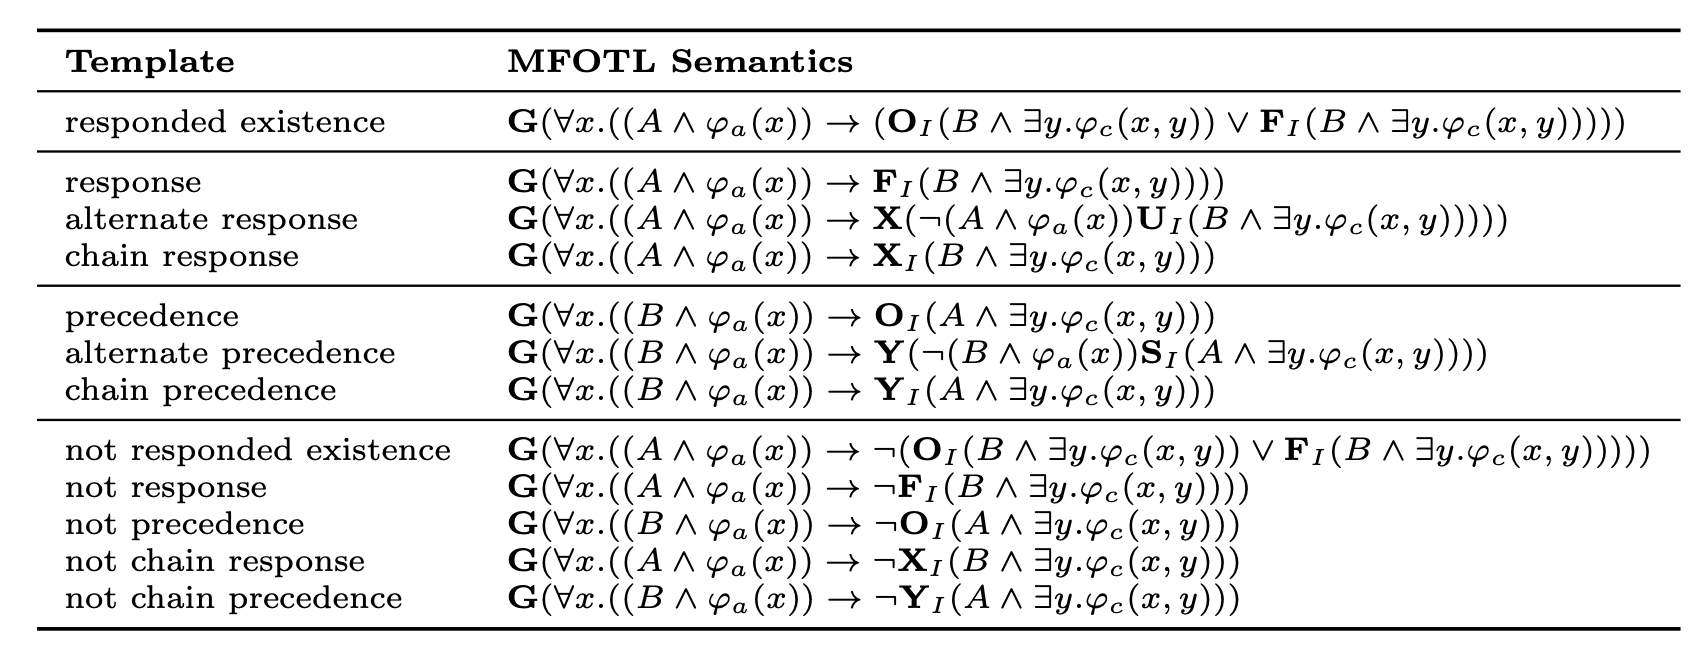
\includegraphics[scale=.3]{figures/mp-declare}
\end{center}



\end{frame}

%------------------------------------------------



\begin{frame}
\frametitle{Previous Work}

\begin{itemize}
	\item Monitoring solved for the propositional case~\cite{}
	\begin{itemize}
		\item Declare is a fragment of LTL on finite traces (LTL$_f$)
		\item Can be catpured by FSA
		\item Technique based on coloring the automaton $\A_\varphi$
		\item Reduces to a fixpoint computation on $\A_\varphi$
	\end{itemize}
\end{itemize}

\begin{itemize}
	\item In general, we are working on lifting the technique to\\ {\bf full MP-Declare}
	\item Currently we are focussing on the {\bf data-only} fragment
\end{itemize}

\end{frame}

%------------------------------------------------

\begin{frame}
\frametitle{Results (ongoing)}

\begin{itemize}	
	\item 
\end{itemize}


\begin{itemize}	
	\item MP-Declare is a sublanguage of LTLf, but we consider the restriction to persistence-preserving
	\item say that we deal with log-traces and that activities have attributes
	\item To perform monitoring we need to compute satisfiability (if we have this, we can always determine all 4 truth values)
	\item We need to establish decidability in this context
	\item We have some results on mu-calc, not directly applicable to LTLf
	\item Our goal is to transfer these results to LTLf (joint work with DC and GDG) 
		and thus to MP-Declare
\end{itemize}

\end{frame}

%------------------------------------------------

\begin{frame}
\frametitle{Results 2}

\begin{itemize}
	\item The results we have are for bounded systems
	\item Declarative PM is a setting where boundedness is a natural assumption
	\item Genericity???? (We should have in the universal TS)
	\item Idea is to prove MC first and then use a universal TS to solve monitoring
		(can do so only if the set of activities is fixed)
	\item Once we have sat, we can encode the prefix and the do monitoring in the standard way
	\item we have to propositionalize everything (with combinatory explosion) then we can use coloring as 
	already dones
	\item Articolo di Riccardo de Masellis per gestire state explosion
	\item Lavori di Demri per data types
	\item Depending on the selected semantics for MP-Declare, LTLf-FOp may be 
		good or not (if we have a set of variables that are changed by the events or not)s
\end{itemize}

\end{frame}

%------------------------------------------------

\end{document} 

\endinput

\begin{frame}
\frametitle{This work}

Main Contributions:
\pause
\begin{itemize}[<+->]
 \item Deductive approach to support transformational  program design and implementation
 \item Automated program synthesis technique with correctness guarantees (wrt spec)
%% \item Link transformational and reactive synthesis
 \item \st{Fully-automated approach from in/out spec to program}
\end{itemize}
~\\


\end{frame}

%------------------------------------------------

\begin{frame}[fragile]
\frametitle{Example: \emph{Size-unbounded} List of int + \emph{register}}

\small

\begin{columns}[t]
	\begin{column}{.4\textwidth} % Left column and width
		Implementation (python)\\~\\

		\tiny
		Some lists:
		\begin{verbatim}
		[8,17,-5,78,13,4,36]
		[7,22,12,40]
		[10,5,13,12,17,-2]
		\end{verbatim}

		\hrule
		
		~\\
		~\\
		
		Operations:
		\begin{verbatim}
		def right() :
			global s
			s += 1

		def update_register() :
			global reg
			reg = list_ex[s]

		def stop() :
			global sc
			sc = True
		\end{verbatim}
		\hrule
		
		~\\
		~\\
		
		Tests:
		\begin{verbatim}
		less_than = list_ex[s] < reg

		at_end = s == len(list_ex)-1
		\end{verbatim}
	\end{column}
	\vrule
	\begin{column}{.55\textwidth} % Left column and width
		High-level spec

		\begin{itemize}
			\item \emph{Operations}\\ (no parameters, use register):
				\begin{itemize}
					\item $right$: moves cursor to the next element
					\item $update\_reg$: copies the value of the current element in the register
					\item $stop$: stops the execution (predefined)
				\end{itemize}
			\item \emph{Tests}:
			\begin{itemize}
				\item $less\_than$: tests if the current element  $<$ value in the register
				\item $at\_end$: tests if at the end of the list 
			\end{itemize}
		\end{itemize}
	\end{column}
\end{columns}

\end{frame}

%------------------------------------------------

\begin{frame}
\frametitle{Example: Find min in List}
	Task:
	\begin{itemize}
		\item Automatic generation of high-level program for minimum in a List 
		\item Transformation into executable (immediate)
	\end{itemize}
	
	~\\
	\pause

	Observations:
	\begin{itemize}[<+->]
		\item List state accessible \emph{only through tests}
		\item Operations \emph{nondeterministic} (end of list is surprise!)
		\item Program: \emph{controller} over List
		\item Goal not observable!
	\end{itemize}
	
	

\end{frame}

%------------------------------------------------


\begin{frame}
\frametitle{Generalized Planning}
	Generalized Planning~{\tiny\cite{srivastava08learning,bonet09automatic,hu:generalized}}:
	\begin{itemize}[<+->]
	\item Instance: (possibly infinite) 
		set of planning domains
		\begin{itemize}
			\item common actions and observations (tests)
			\item e.g.: lists
		\end{itemize}
	\item Task: Find plan for \emph{reachability goal}
		\begin{itemize}
			\item e.g.: reach end of list
		\end{itemize}
	\item Same plan for \emph{all planning domains}
		\begin{itemize}
			\item must use common actions and observations
		\end{itemize}
	\item Assumption: \emph{goal is observable!}
	\end{itemize}
\end{frame}

%------------------------------------------------


\begin{frame}
\frametitle{Generalized Planning}

Typically solved by reduction to FOND planning~{\tiny\cite{bonet:ijcai2017}}:
	\begin{itemize}[<+->]
	\item FOND domain is \emph{observation abstraction} of \emph{all} planning domains
		\begin{itemize}
		 \item E.g., if not at end can move right
		 \item if move right, next either at end or not
		\end{itemize}

	\item Nondeterminism models uncertainty over observations
	\item Nondeterministic	effects are \emph{fair}
		\begin{itemize}
			\item infinitely many executions of an action 
				imply occurrence of all effects
			\item if move right infinitely many times,
			eventually at end
		\end{itemize}
	\item Solutions are policies (stateless controllers): observations $\rightarrow$ action
		\begin{itemize}
			\item Strongly cyclic solutions: 
				goal-reaching on fair traces
			\item e.g.: move right until end observed
		\end{itemize}
	\end{itemize}
	
\end{frame}

%------------------------------------------------

\begin{frame}
\frametitle{Generalized Planning and Program Synthesis}


SIMILARITIES
\begin{itemize}[<+->]
	\item Conceptually analogous: one solution for all
	\item Can see underlying instances as planning domains
		(common actions and observations)
\end{itemize}
	
~\\
\pause
	
CRUCIAL DIFFERENCES
	\begin{itemize}[<+->]
	\item Goal is {\bf NOT observable}
		\begin{itemize}
			\item find min, but $min$ cannot be sensed
		\end{itemize}
	\item Goal is {\bf NOT reachability}
		\begin{itemize}
			\item min found if controller 
				satisfies \emph{execution requirements} (see below)
		\end{itemize}
	\item Controller is {\bf stateful}
	\end{itemize}

\pause	
\begin{center}
 Generalized (and FOND) planning not powerful enough!
\end{center}
	
\end{frame}

% ------------------------------------------------

\begin{frame}[fragile]
\frametitle{Execution Requirements}
\framesubtitle{Beyond reachability and goal observablity}

\begin{itemize}[<+->]
 \item Goal not observable: cannot test goal achievement
 
 \item Goal achievement is consequence of controller execution
	\begin{itemize}
		\item must fulfill \emph{Execution Requirements}
		\item Part of controller's goal
	\end{itemize}
\end{itemize}


\pause

\begin{block}{Execution Requirement}
Temporal constraints over executions, e.g.:

\begin{itemize}
	\item {\bf ALWAYS 
     (update register iff current value less than register)}
\end{itemize}



Guarantees that: {\bf (at end) $\rightarrow$  (min stored in register)}

~\\

(Assume start at leftmost cell)

\end{block}

\end{frame}

% ------------------------------------------------

\begin{frame}[fragile]
\frametitle{Execution Requirements}
\framesubtitle{Beyond reachability and goal observablity}

Execution requirements:
\begin{itemize}[<+->]
	\item Designer responsibility
	\item Hard to come up with $\rightarrow$ possibly as much as traditional program
\end{itemize}

\pause
~\\

Advantages:
\begin{itemize}[<+->]
	\item Work at solution logic level
	\item Bugs cannot stem from implementation details
\end{itemize}

\end{frame}

%------------------------------------------------

\begin{frame}
\frametitle{LTL Synthesis}

LTL (Reactive) Synthesis (intuition):
\begin{itemize}[<+->]
	\item Given an LTL temporal specification $\varphi$
	\item Synthesize a controller that satisfies $\varphi$
	\item (specific setting with input/output propositions required)
\end{itemize}

\pause

\begin{center}
FOND + (fairness) + (temporal goal) solvable as \emph{LTL synthesis}
\end{center}

~\\

\begin{center}
\bf Can synthesize transformational programs using LTL synthesis!
\end{center}


\end{frame}

%------------------------------------------------

\begin{frame}
\frametitle{Program Synthesis as \emph{LTL synthesis}}

LTL specification:
%%Declarative pseudocode specification

\[\varphi=Pre\land ((Eff  \land Fair) \rightarrow Goal)\]

\pause

\begin{itemize}[<+->]
	\item $Pre$: Action preconditions of observation abstraction (systematic)
	\item $Eff$: Action effects+frame+init of observation abstraction (systematic)
	\item $Fair$: Fairness assumptions (manual, designer, requires creativity, usually easy)
	\item $Goal$: controller's  goal, includes exec reqs\\ (manual, designer, requires creativity, typically hard)
\end{itemize}

\pause
Observation:
\begin{itemize}
 \item $Goal$:  includes exec reqs and ``essence'' of program to synthesize\\ 
 (solution requirement)
\end{itemize}



\end{frame}

%------------------------------------------------

\begin{frame}
\frametitle{Program Synthesis as \emph{LTL synthesis}}
\framesubtitle{Example}

\[\varphi=Pre\land ((Eff  \land Fair) \rightarrow Goal)\]

  \small
  \begin{itemize}[<+->]
  \item $Pre$:
    $\begin{array}{l}
       \always (\mathit{right} \limp \lnot \mathit{at\_end}) \land {}\\
     \always (\mathit{right} \;xor\; \mathit{update\_reg} \;xor\; \mathit{stop}) \land
       \always (\mathit{stop} \limp\nextX \mathit{stop})
     \end{array}
     $
 
  \item $Eff$:
    $\begin{array}{l}
       \always(\mathit{update\_reg} \limp \nextX \lnot \mathit{less\_than} \land pers(\mathit{at\_end}))\land {}\\
       \always(\mathit{stop} \limp pers(\mathit{at\_end}) \land pers(\mathit{less\_than}))
     \end{array}
     $

\item $Fair$: 
	$\begin{array}{l}
		\always\, \eventually \mathit{right} \limp \eventually \mathit{at\_end}
	\end{array}
	$
\item $Goal$:
	$\begin{array}{l}
       \eventually\, \always\mathit{at\_end} \land {}\\
		\always(\mathit{less\_than} \equiv \mathit{update\_reg})
     \end{array}
     $
\end{itemize}

\end{frame}

%------------------------------------------------

\begin{frame}[fragile]
\frametitle{Program Synthesis as \emph{LTL synthesis}}
\framesubtitle{Example, cont'd}
\small
LTL synthesis engine \textsc{strix} (\url{strix.model.in.tum.de/try/})

\begin{verbatim}
G((r & !s & !u) || (!r & s & !u) || (!r & !s & u)) & G(s -> X(s))
G(r -> !e)
(G(u -> (X(!lt) & (e <-> X(e)))) & 
 G(s -> ((e <-> X(e)) & (lt <-> X(lt)))) & G(F(r)) -> F(e)) ->
               (F(G(e)) & G(lt <-> u))

input: e, lt  output: r, s, u
\end{verbatim}

\begin{center}
	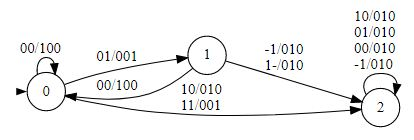
\includegraphics[width=.5\textwidth]{figures/automata_min_list_for_notebook}
\end{center}
\vspace{-2ex}
\hfill $\mathit{at\_end},\, \mathit{less\_than} \;/\; \mathit{right},\, \mathit{stop},\, \mathit{update\_reg}$



\end{frame}

%------------------------------------------------

\begin{frame}[fragile]
\frametitle{Program Synthesis as \emph{LTL synthesis}}
\framesubtitle{Example, cont'd}
  \footnotesize
	\begin{columns}[t]
	\begin{column}{0.45\textwidth}
  Controller code (automatic)
  \tiny
\begin{verbatim}
while not(sc):
        #acting according to strategy
        if(currState==0) :
            if (not(at_end) and not(less_than)): 
                right()
                currState = 0
            if (not(at_end) and less_than): 
                update_register()
                currState = 1
            if (at_end and less_than): 
                update_register()
                currState = 2
            if (end and not(less_than)): 
                stop()
                currState = 2
        elif(currState == 1) :
            if (not(at_end) and not(less_than)): 
                right()
                currState = 0
            if(less_than or at_end):
                right()
                currState=2
        elif(currState == 2) :
            stop()
            currState=2
\end{verbatim}
 
\end{column}
\begin{column}{0.45\textwidth}
 Run on concrete list:
 \tiny
\begin{verbatim}
List:  [8, 17, -5, 78, 13, 4, 36]
Action performed: right
Action performed: right
Action performed: update_register
Action performed: right
Action performed: right
Action performed: right
Action performed: right
Action performed: stop
Minimum value of the list: -5

List:  [7, 22, 12, 40]
Action performed: right
Action performed: right
Action performed: right
Action performed: stop
Minimum value of the list: 7

List:  [10, 5, 13, 12, 17, -2]
Action performed: right
Action performed: update_register
Action performed: right
Action performed: right
Action performed: right
Action performed: right
Action performed: update_register
Action performed: stop
Minimum value of the list: -2

\end{verbatim}
 % List:  [99]
% Action performed: stop
% Minimum value of the list: 99
\end{column}
\end{columns}
% 
\end{frame}

%------------------------------------------------

\begin{frame}
\frametitle{Summary of the Approach}

\begin{center}
	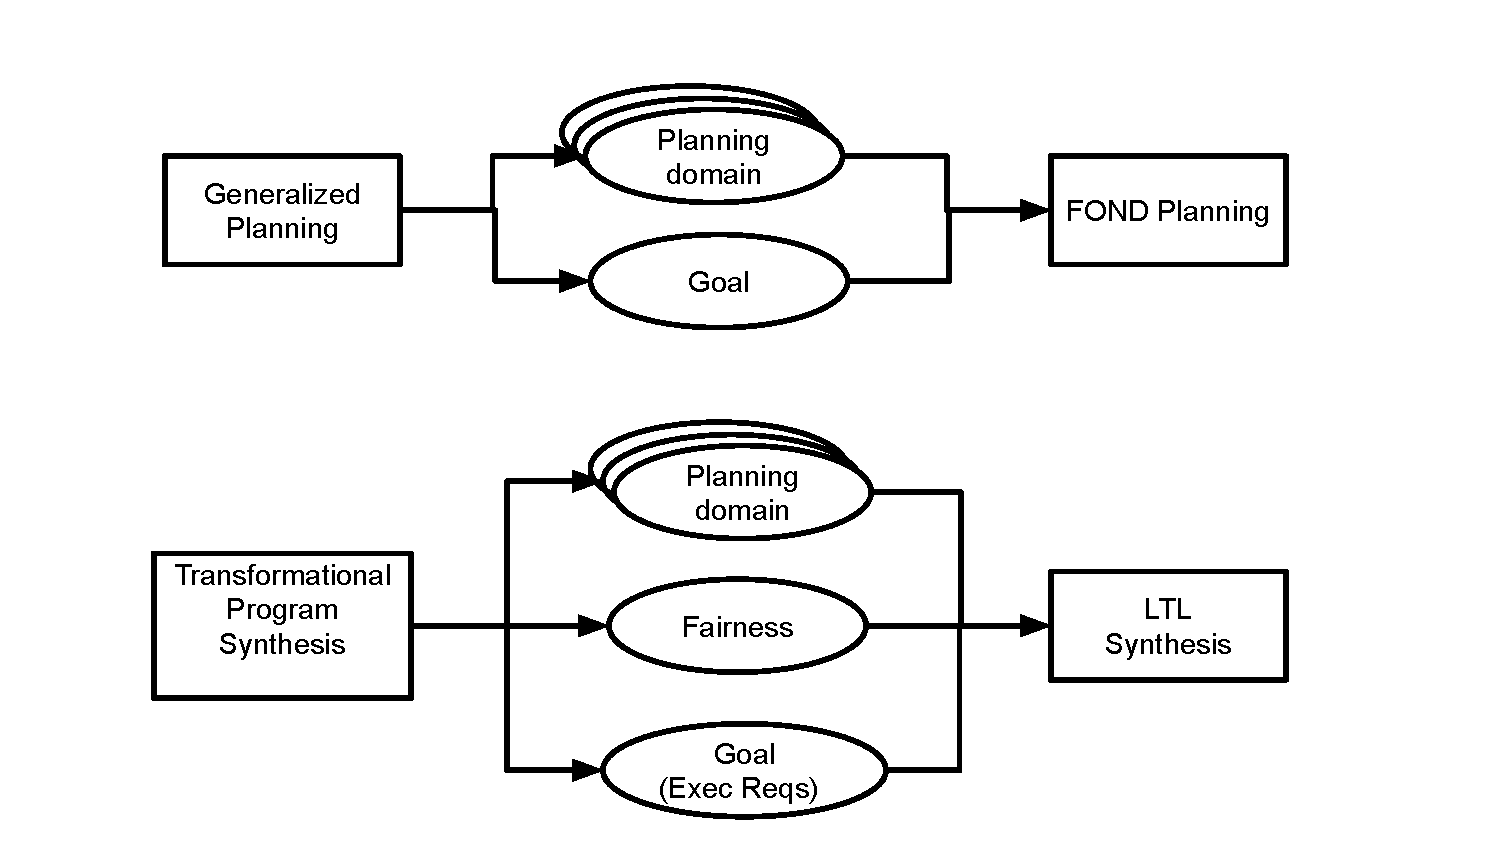
\includegraphics[scale=.5]{figures/diagram}
\end{center}

\end{frame}

%------------------------------------------------

\begin{frame}
\frametitle{Some Experiments}

Approach successfully tested 
with\footnote{Implementation by master students E. Cicero, 
D.~Giunta, L.~Pierdicca.}:

\begin{itemize}
	\small
	\item List traversal (paper)
	\item Doubly-linked list traversal (paper)
	\item Binary tree traversal (paper)
	\item Graph traversal (paper)
	\item min/max in list (paper)
	\item Tree membership (paper)
	\item Copy even numbers in another list
	\item Sum of positive numbers of a list
	\item Bubble sort
	\item Robot navigation to position in a matrix 
\end{itemize}  

All solutions in paper obtained in $<10$s using 
\textsc{ Strix} online demo version 
\end{frame}

%------------------------------------------------

\begin{frame}
\frametitle{Conclusions}

\begin{itemize}[<+->]
	\item A logic-based deductive approach to support designers/programmers
		\begin{itemize}
			\item Correctness guarantee
		\end{itemize}

	\item Semi-automated program synthesis technique
		
	\item Requires \emph{creativity}:
		\begin{itemize}
			\item Fairness assumptions
			\item Execution requirements (and goal)
% 			\emph{logical} constraints on 
% 				\emph{traces} controller induces/considers
		\end{itemize}
		
	\item Advantages:
	\begin{itemize}
		\item Focus on solution logic, not on implementation details
		\item Confination of bug sources
	\end{itemize}
		
	\item Amenable to automated reasoning (not this paper)
	
\end{itemize}

\end{frame}

%------------------------------------------------

\begin{frame}
\frametitle{Future Work}

\begin{itemize}[<+->]
	\item Improve performance/scalability:
		\begin{itemize}
			\item \emph{Planning instead of full-fledged LTL synthesis}
			\item e.g., focus on LTLf goals 
				under assumptions 
				(such as fairness in FOND)
		\end{itemize}
	\item Modularity: if/how specifications can be combined?
		\begin{itemize}
		\item e.g., min in list is list traversal with 
			different execution requirements
		\end{itemize}
\end{itemize}

\end{frame}

%------------------------------------------------

\begin{frame}
\Huge{
	\centerline{Thanks for the Attention!}
	~\\
	\centerline{Q\&A}
}

\end{frame}

%------------------------------------------------

\begin{frame}[allowframebreaks]
\frametitle{References}
\tiny{
% \begin{thebibliography}{99} % Beamer does not support BibTeX so references must be inserted manually as below
% \bibitem[Smith, 2012]{p1} John Smith (2012)
% \newblock Title of the publication
% \newblock \emph{Journal Name} 12(3), 45 -- 678.
% \end{thebibliography}
\bibliographystyle{amsalpha}
\bibliography{control,control2}
}
\end{frame}

%----------------------------------------------------------------------------------------
